\PassOptionsToPackage{unicode=true}{hyperref} % options for packages loaded elsewhere
\PassOptionsToPackage{hyphens}{url}
%
\documentclass[]{article}
\usepackage{lmodern}
\usepackage{amssymb,amsmath}
\usepackage{ifxetex,ifluatex}
\usepackage{fixltx2e} % provides \textsubscript
\ifnum 0\ifxetex 1\fi\ifluatex 1\fi=0 % if pdftex
  \usepackage[T1]{fontenc}
  \usepackage[utf8]{inputenc}
  \usepackage{textcomp} % provides euro and other symbols
\else % if luatex or xelatex
  \usepackage{unicode-math}
  \defaultfontfeatures{Ligatures=TeX,Scale=MatchLowercase}
\fi
% use upquote if available, for straight quotes in verbatim environments
\IfFileExists{upquote.sty}{\usepackage{upquote}}{}
% use microtype if available
\IfFileExists{microtype.sty}{%
\usepackage[]{microtype}
\UseMicrotypeSet[protrusion]{basicmath} % disable protrusion for tt fonts
}{}
\IfFileExists{parskip.sty}{%
\usepackage{parskip}
}{% else
\setlength{\parindent}{0pt}
\setlength{\parskip}{6pt plus 2pt minus 1pt}
}
\usepackage{hyperref}
\hypersetup{
            pdfborder={0 0 0},
            breaklinks=true}
\urlstyle{same}  % don't use monospace font for urls
\usepackage{graphicx,grffile}
\makeatletter
\def\maxwidth{\ifdim\Gin@nat@width>\linewidth\linewidth\else\Gin@nat@width\fi}
\def\maxheight{\ifdim\Gin@nat@height>\textheight\textheight\else\Gin@nat@height\fi}
\makeatother
% Scale images if necessary, so that they will not overflow the page
% margins by default, and it is still possible to overwrite the defaults
% using explicit options in \includegraphics[width, height, ...]{}
\setkeys{Gin}{width=\maxwidth,height=\maxheight,keepaspectratio}
\setlength{\emergencystretch}{3em}  % prevent overfull lines
\providecommand{\tightlist}{%
  \setlength{\itemsep}{0pt}\setlength{\parskip}{0pt}}
\setcounter{secnumdepth}{0}
% Redefines (sub)paragraphs to behave more like sections
\ifx\paragraph\undefined\else
\let\oldparagraph\paragraph
\renewcommand{\paragraph}[1]{\oldparagraph{#1}\mbox{}}
\fi
\ifx\subparagraph\undefined\else
\let\oldsubparagraph\subparagraph
\renewcommand{\subparagraph}[1]{\oldsubparagraph{#1}\mbox{}}
\fi

% set default figure placement to htbp
\makeatletter
\def\fps@figure{htbp}
\makeatother


\date{}

\begin{document}

\hypertarget{projecte-asix-2k22}{%
\section{\texorpdfstring{\textbf{Projecte ASIX
2k22}}{Projecte ASIX 2k22}}\label{projecte-asix-2k22}}

\hypertarget{escola-del-treball}{%
\subsection{\texorpdfstring{\textbf{Escola Del
Treball}}{Escola Del Treball}}\label{escola-del-treball}}

\hypertarget{hisx-2021-2022}{%
\subsubsection{\texorpdfstring{\textbf{2HISX
2021-2022}}{2HISX 2021-2022}}\label{hisx-2021-2022}}

\hypertarget{aaron-andal-cristian-condolo}{%
\subsubsection{\texorpdfstring{\textbf{Aaron Andal \& Cristian
Condolo}}{Aaron Andal \& Cristian Condolo}}\label{aaron-andal-cristian-condolo}}

\hypertarget{cryptosec-careful-where-you-step-in}{%
\section{\texorpdfstring{\textbf{CryptoSEC}: ``\emph{Careful where you
step
in}''}{CryptoSEC: ``Careful where you step in''}}\label{cryptosec-careful-where-you-step-in}}

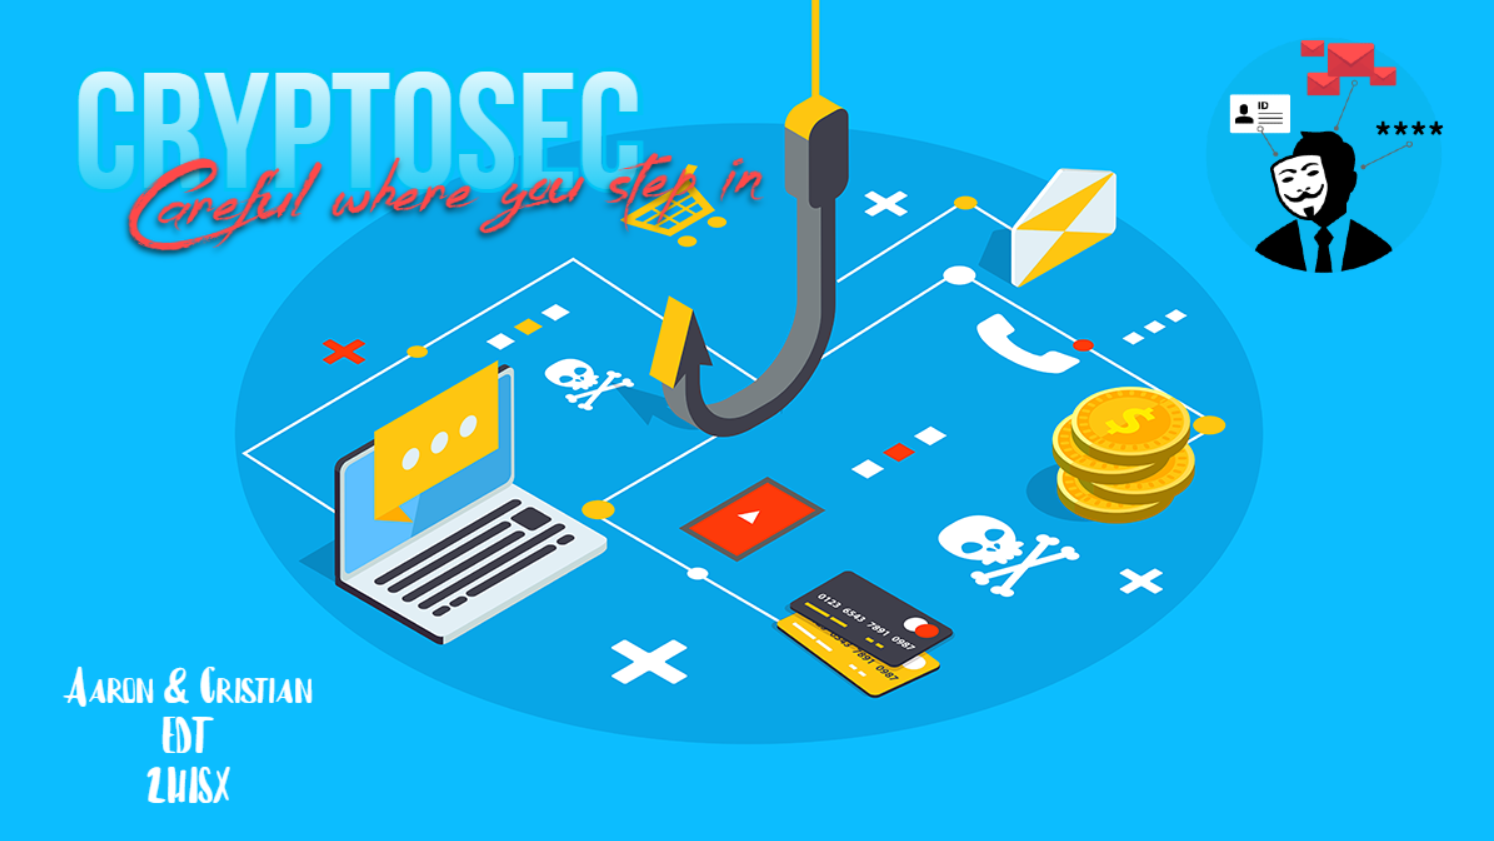
\includegraphics{./tex2pdf.-0711d24f439ae21b/785b57206d80bd3d5ef15f036481e103db8435a1.png}

\hypertarget{index}{%
\section{\texorpdfstring{\textbf{Index}}{Index}}\label{index}}

\begin{itemize}
\item
  \textbf{DNS}: \href{}{--\textgreater{} readME \textless{}--}
\item
  \textbf{DNSSEC}: \href{}{--\textgreater{} readME \textless{}--}
\item
  \textbf{DNS}: \href{}{--\textgreater{} readME \textless{}--}
\item
  \textbf{DNSSEC}: \href{}{--\textgreater{} readME \textless{}--}
\end{itemize}

\hypertarget{deployment}{%
\section{Deployment}\label{deployment}}

\hypertarget{requisits}{%
\subsection{Requisits:}\label{requisits}}

\hypertarget{virtualitzaciuxf3}{%
\subsubsection{\texorpdfstring{\textbf{Virtualització}}{Virtualització}}\label{virtualitzaciuxf3}}

\begin{itemize}
\tightlist
\item
  {[} {]} 1 SOA
\item
  {[} {]} 1 Forwarder
\item
  {[} {]} 2 Kali
\item
  {[} {]} 3 Clients en Xarxa Interna
\end{itemize}

\hypertarget{programari-cryptosec}{%
\subsubsection{\texorpdfstring{\textbf{Programari
CryptoSEC}}{Programari CryptoSEC}}\label{programari-cryptosec}}

\begin{itemize}
\tightlist
\item
  {[} {]} NETPLAN --\textgreater{} Configuración Network Manager dels
  Servidors Ubuntu Server.
\item
  {[} {]} NMAP --\textgreater{} Verificació d'arp, ports\ldots{} etc.
\item
  {[} {]} BIND9 --\textgreater{} Forwarder i SOA han de poder resoldre
  peticions DNS als clients.
\item
  {[} {]} DHCP --\textgreater{} Xarxa Interna --\textgreater{}
  Configuració automàtica IP i DNS.
\item
  {[} {]} IPTABLES --\textgreater{} Xarxa Interna --\textgreater{} NAT a
  l'exterior.
\item
  {[} {]} APACHE2 --\textgreater{} https://cryptosec.net
\item
  {[} {]} TEAMVIEWER --\textgreater{} GUI remot
\item
  {[} {]} SSH --\textgreater{} Accés remot
\item
  {[} {]} OPENVAS --\textgreater{} Verificació de vulnerabilitats
\item
  {[} {]} WIRESHARK --\textgreater{} Analitzador de paquets del sistema
\item
  {[} {]} ARP -A --\textgreater{} Veure taula CACHE
\item
  {[} {]} HOST --\textgreater{} Resolver
\item
  {[} {]} NSLOOKUP --\textgreater{} Resolver
\item
  {[} {]} DIG --\textgreater{} Resolver
\item
  {[} {]} JOURNALCTL --\textgreater{} Veure possibles errors
\item
  {[} {]} SYSTEMCTL --\textgreater{} Reiniciar o reload dels serveis
\item
  {[} {]} SSL --\textgreater{} Certificats per Apache2
\item
  {[} {]} ROUTING --\textgreater{} Per poder entrar a 192.168.3.0/24
  desde la classe.
\item
  {[} {]} TRACEROUTE --\textgreater{} Observar el traçat del paquet.
\item
  {[} {]} PING --\textgreater{} Observar la conectivitat entre
  dispositius.
\item
  {[} {]} CERTBOT - LET'S ENCRYPT --\textgreater{} Generar certificats
  per dominis reals (\emph{Tried}).
\item
  {[} {]} WAZUH --\textgreater{} Detectar vulnerabilitats del sistema i
  de la xarxa (\emph{Tried}).
\end{itemize}

\hypertarget{hacking-kali}{%
\subsubsection{\texorpdfstring{\textbf{HACKING
Kali}}{HACKING Kali}}\label{hacking-kali}}

\begin{itemize}
\tightlist
\item
  {[} {]} SET --\textgreater{} Setoolkit --\textgreater{} Software
  d'atacs d'Enginyeria Social
\item
  {[} {]} BETTERCAP --\textgreater{} Framework/Sniffer per poder fer
  atacs de Man in the Middle.
\item
  {[} {]} ZPHISHING --\textgreater{} Framework per simular
  \emph{Phishing} real.
\item
  {[} {]} ETTERCAP --\textgreater{} Framework/Sniffer per poder fer
  atacs de man in the Middle.
\item
  {[} {]} JOHN --\textgreater{} Brute Force Attack tool --\textgreater{}
  Cracker password
\item
  {[} {]} SSLSTRIP --\textgreater{} Strips HTTPS to HTTP (\emph{Tried})
\item
  {[} {]} SLOWHTTP --\textgreater{} A type of DOS to take down
  \textbf{cryptosec.net} (\emph{Tried})
\end{itemize}

\hypertarget{practica}{%
\section{\texorpdfstring{\textbf{Practica:}}{Practica:}}\label{practica}}

\includegraphics{./tex2pdf.-0711d24f439ae21b/435c2dc624a5342e23e6fe2aae43e04e8c80f8a6.png}

\hypertarget{plantejament-a-virtualbox}{%
\subsection{\texorpdfstring{\textbf{Plantejament a
VIRTUALBOX}:}{Plantejament a VIRTUALBOX:}}\label{plantejament-a-virtualbox}}

\hypertarget{portuxe0til-den-keshi}{%
\subsubsection{\texorpdfstring{\textbf{Portàtil d'en
Keshi}:}{Portàtil d'en Keshi:}}\label{portuxe0til-den-keshi}}

\begin{itemize}
\item
  \begin{itemize}
  \item
    Kali Linux: BRIDGE (DHCP eth0)

    \begin{itemize}
    \item
      X11 Forwarding SSH o Teamviewer
    \item
      Static Routing to 192.168.3.0/24: ip route add 192.168.3.0/24 via
      10.200.243.168 dev eno1
    \item
      Setoolkit
    \item
      Ettercap
    \item
      Bettercap
    \item
      John (Brute Force Crack)
    \item
      Wireshark
    \item
      Nmap
    \item
      Traceroute
    \end{itemize}
  \end{itemize}
\end{itemize}

\hypertarget{portuxe0til-den-cristian}{%
\subsubsection{\texorpdfstring{\textbf{Portàtil d'en
Cristian}:}{Portàtil d'en Cristian:}}\label{portuxe0til-den-cristian}}

\begin{itemize}
\item
  \begin{itemize}
  \tightlist
  \item
    KALI White Hacker
  \end{itemize}
\end{itemize}

\begin{verbatim}
- Ub 20.04 SOA "SOACryptosec": BRIDGE (DHCP enp0s3) - 10.200.243.164/24

    - APACHE2: Pàg www.cryptosec.net o 10.200.243.164/cryptosec/index.html

        - /var/www/html/cryptosec/index.html

        - Perquè funcioni el HTTPS cal importar el CACERT.PEM al FIREFOX.

    - DNS AUTORITARI (cryptosec.net)

        - DNS

        - DNSSEC
\end{verbatim}

\hypertarget{pc-aaron-i11}{%
\subsubsection{\texorpdfstring{\textbf{PC Aaron
i11}:}{PC Aaron i11:}}\label{pc-aaron-i11}}

\begin{itemize}
\item
  \begin{itemize}
  \item
    Ub 20.04 Forwarder ``ForwarderCryptosec'':

    \begin{itemize}
    \item
      BRIDGE (DHCP enp0s3) - 10.200.243.168/24
    \item
      Internal Network (cryptosec enp0s8 192.168.3.0/24) -
      192.168.3.1/24
    \item
      IPTABLES
    \item
      DHCP
    \item
      DNS FORWARDING
    \end{itemize}
  \item
    Cryptosec Clients:

    \begin{itemize}
    \tightlist
    \item
      Internal Network (cryptosec enp0s3 192.168.3.0/24) -
      192.168.3.100/24 ​​- 192.168.3.200/24
    \end{itemize}
  \end{itemize}
\end{itemize}

\hypertarget{kali-keshi-hacker}{%
\subsubsection{\texorpdfstring{\textbf{Kali
(Keshi-Hacker)}}{Kali (Keshi-Hacker)}}\label{kali-keshi-hacker}}

\begin{enumerate}
\def\labelenumi{\arabic{enumi}.}
\item
  Verificació de les IPS i conectivitat amb Internet.
\item
  Rebre la IP per DHCP de la classe.
\item
  Activar services.sh.
\item
  Activar Teamviewer o cctivar X11 Forwarding SSH a l'ordinador del
  Professor:
\end{enumerate}

\emph{Extra}

X11 FORWARDING (Permetre Obrir Apps mode Gràfic):

\begin{verbatim}
- ssh -X anonymous@ip

- xauth list $DISPLAY --> COPIAR1

- fet $DISPLAY --> COPIAR2

- sudo bash

- xauth add [ENGANXAR COPIAR1]

- export DISPLAY=[ENGANXAR COPIAR2]
\end{verbatim}

\begin{enumerate}
\def\labelenumi{\arabic{enumi}.}
\setcounter{enumi}{4}
\tightlist
\item
  Verificar conectivitat des de l'ordinador del PROFE i veure què es pot
  obrir OK.
\end{enumerate}

\begin{center}\rule{0.5\linewidth}{0.5pt}\end{center}

\hypertarget{soa}{%
\subsubsection{\texorpdfstring{\textbf{SOA}}{SOA}}\label{soa}}

\begin{enumerate}
\def\labelenumi{\arabic{enumi}.}
\item
  Verificació de les IPS i conectivitat amb Internet.
\item
  Modificar \textbf{NETPLAN}.

  \begin{itemize}
  \item
    netplan try + netplan apply
  \item
    IMPORTANT! Verificar \emph{PING} i \emph{RESOLV} cryptosec.net amb
    la IP adequada!
  \end{itemize}
\item
  Modificar BIND9 (Primer en \textbf{DNS normal} i després
  \textbf{DNSSEC}).
\item
  Verificar \textbf{APACHE2}: 10.200.243.164 i
  10.200.243.164/cryptosec/index.html

  \begin{itemize}
  \item
    Verificar els fitxers de \textbf{``cryptosec.net''} a Apache2

    \begin{itemize}
    \item
      Són a \textbf{/etc/apache2/sites-available/cryptosec.net.conf}
    \item
      Comandes per verificar Apache2:

      \begin{itemize}
      \item
        \textbf{a2ensite cryptosec.net.conf} --\textgreater{} Habilita
        els virtualHost.
      \item
        \textbf{apache2ctl configtest} --\textgreater{} Verifica apache2
      \item
        \textbf{openssl x509 --noout --text -in cacert.pem}
      \item
        \textbf{openssl x509 --noout --text -in cryptosec\_cert.pem}
      \item
        \textbf{ufw allow ``Apache Full''} --\textgreater{} Permet
        firewall Apache2
      \end{itemize}
    \end{itemize}
  \end{itemize}
\item
  Verificar que \textbf{DNSSEC} funciona:

  \begin{itemize}
  \item
    \textbf{dnssec-keygen} --\textgreater{} GENERAR
  \item
    \textbf{\$INCLUDE a db.cryptosec.net} --\textgreater{} Signatura
    manual
  \item
    \textbf{dnssec-signzone} --\textgreater{} Signar autom .signed
  \item
    \textbf{dig cryptosec.net +dnssec +multiline}
  \item
    \textbf{dnssec-verify -o cryptosec.net db.cryptosec.net {[}-v
    level{]}}
  \item
    \textbf{host cryptosec.net}
  \item
    \textbf{nslookup cryptosec.net}
  \end{itemize}
\item
  Verificar claus de \textbf{DNSSEC} i engegada davant \textbf{spoofing}
  de la zona.
\end{enumerate}

\hypertarget{forward}{%
\subsubsection{\texorpdfstring{\textbf{FORWARD}}{FORWARD}}\label{forward}}

\begin{enumerate}
\def\labelenumi{\arabic{enumi}.}
\item
  Verificació de les \textbf{IPS} i conectivitat amb Internet.
\item
  Modificar NETPLAN.

  \begin{itemize}
  \item
    netplan try + netplan \textbf{apply}.
  \item
    IMPORTANT! Verificar PING i RESOLV cryptosec.net amb la IP adequada!
  \item
    Verificar que el DNS nameserver sigui FORWARDER a
    \textbf{10.200.243.164}.
  \end{itemize}
\item
  Activar IPTABLES: \textbf{cryptonat.sh}

  \begin{itemize}
  \tightlist
  \item
    Verificar ip estàtica de la classe \textbf{10.200.243.168}.
  \end{itemize}
\item
  Activar \textbf{FORWARDING de DNS}.

  \begin{itemize}
  \item
    Verificar \textbf{named.conf.default-zones}
  \item
    Ver \textbf{named.conf.options}
  \item
    Reiniciar i verificar que facin PING I RESOLV. Sinó Journal.
  \end{itemize}
\item
  Activar \textbf{DHCP} per a \texttt{192.168.3.0} \emph{barra} 24 a la
  interfície \textbf{enp0s8}.

  \begin{itemize}
  \item
    Reiniciar DHCP i verificar.
  \item
    Fitxers \textbf{/etc/dhcp/dhcpd.conf} i
    \textbf{/etc/default/isc-dhc-server}
  \item
    Verificar amb CLIENTS que rebin la IP i facin resoldre a
    cryptosec.net.
  \end{itemize}
\end{enumerate}

\hypertarget{clients}{%
\subsubsection{\texorpdfstring{\textbf{CLIENTS}}{CLIENTS}}\label{clients}}

\begin{enumerate}
\def\labelenumi{\arabic{enumi}.}
\item
  Obrir i verificar que rebin IP i DNS.

  \begin{itemize}
  \item
    Sinó reiniciar networking o dhclient -r (\emph{release}) i dhclient
    -v (\emph{verbose}).
  \item
    Al FIREFOX introduir el cacert.pem --\textgreater{} Importar al
    navegador i provar https://cryptosec.net
  \item
    \textbf{LINUX}: systemd-resolve \textbf{--flush-cache}
    --\textgreater{} Neteja la cahcé DNS
  \item
    \textbf{Windows}: ipconfig \textbf{/flushdns}
  \end{itemize}
\end{enumerate}

\hypertarget{comander-per-verificar-la-conectivitat}{%
\subsubsection{\texorpdfstring{\textbf{Comander per verificar la
conectivitat}:}{Comander per verificar la conectivitat:}}\label{comander-per-verificar-la-conectivitat}}

\begin{verbatim}
- systemd-resolved --status --> Verifica DNS actual

- nmap -sP 10.200.243.0/24 --> Escaneig de la Xarxa

- resolvectl query cryptosec.net --> Resol cryptosec.net

- host cryptosec.net --> Resol cryptosec.net

- dig cryptosec.net +dnssec +multiline --> Resol cryptosec.net segur DNSSEC.
\end{verbatim}

\begin{itemize}
\item
  \textbf{EXTRES}:

  \begin{itemize}
  \item
    Ordinador PROFE fer ROUTING a 192.168.3.0/24

    \begin{itemize}
    \item
      Han de tenir NAT a l'exterior (Forwarder ha d'activar Iptables)
    \item
      ip route add 192.168.3.0/24 via 10.200.243.168 dev eno1
    \item
      Provar PING

      \begin{itemize}
      \tightlist
      \item
        Provar SSH -X usuariClientCryptosec@192.168.3.x
      \end{itemize}
    \end{itemize}
  \end{itemize}
\end{itemize}

X11 FORWARDING (Permetre Obrir Apps mode Gràfic):

\begin{verbatim}
- ssh -X anonymous@ip

- xauth list $DISPLAY --> COPIAR1

- fet $DISPLAY --> COPIAR2

- sudo bash

- xauth add [ENGANXAR COPIAR1]

- export DISPLAY=[ENGANXAR]
\end{verbatim}

\hypertarget{atacs-del-hacker}{%
\section{\texorpdfstring{\textbf{Atacs del
hacker}}{Atacs del hacker}}\label{atacs-del-hacker}}

\begin{itemize}
\item
  \textbf{Brute Force Attack - Cracking Password with John}: El hacker
  ha aconseguit una copia dels fitxers /etc/passwd i /etc/shadow i les
  ha anomenat mini-passwd.txt i mini-shadow.txt. John és un
  \textbf{tool} de Kali que permetrà desxifrar els \emph{hashes} de les
  contrasenyes. Quant més difícil més temps trigarà. Posarem
  contrasenyes sencilletes. Podrem veure com les desxifra. Utilitzarà un
  diccionari \textbf{rockyou.txt}. Aprofitant també que l'usuari ha
\item
  \textbf{ARP Poisoning / Spoofing (2 parts) (BETTERCAP)}: Envenenament
  de les taules ARP de les víctimes implicades i reenviament de paquets
  al hacker. Amb el Wireshark - ARP - Nmap, veurem com fa el duplicat de
  MAC.

  \begin{itemize}
  \item
    \textbf{MITM - Eavesdropping (Sniffing) (BETTERCAP)}: Amb l'ARP
    Spoof d'abans activarem un \emph{sniffer} i estarem escoltant la
    màquina afectada i veient les pàgines on visita. Podem captar
    credencials de pàgines HTTP.
  \item
    \textbf{DNS Poisoning / Spoofing) (BETTERCAP)}: Amb l'ARP Spoof
    d'abans activarem un \emph{dnsspoof} i injectarem un registre de DNS
    fals on ens redirigirà a la nostra màquina on hi tindrem una
    \emph{fake page: m0odle.escoladeltreball.org} (\textbf{Moodle EDT})
    i l'enviarem per correu utilitzant \textbf{SET} dient que
    ``\emph{URGENT! L'Eduard ha posat les notes de M06, entra urgentment
    i mira la nota que tens!!!}'' llavors l'usuari entrarà i no se
    n'adonarà i li robarem les credencials mostrades al \textbf{SET}.
  \end{itemize}
\item
  \textbf{Spoofing CryptoSEC.NET + DOS SlowHTTP (take down
  cryptosec.net) (BETTERCAP)}: Ídem que l'anterior però els targets son
  el \textbf{SOA} i el \textbf{Forwarding}, els clients interns de
  CryptoSEC quan hagin d'anar a la pàgina web \textbf{cryptosec.net},
  entraràn a \textbf{cryptos3c.net} ja que el hacker ha avisat que hi hà
  una urgència a la pàgina principal i han d'entrar a la pàgina web dada
  pel hacker i les seves credencials seràn \textbf{robades sense que
  se'n adoni}! Abans de tot, el hacker utilitzarà una eina per que la
  pàgina de \textbf{cryptosec.net} vagi més lent durant uns minuts.
  Durant aquest minuts aprofitarà per donar un comunicat oficial a
  l'empresa CryptoSEC dient que la pàgina ha sigut tumbada i han d'anar
  a un altra anomenada \texttt{cryptos3c.net}.
\item
  \textbf{ZPHISHING: Phishing with a real ``fake'' HTTPS website}:
  Exemple real de \textbf{Phishing} automatitzat i desplegat a
  \textbf{Cloudflare} per un programa anomenat \textbf{Zphishing}.
  Genera servidor temporal a Internet amb una plantilla a escollir de
  l'usuari. Enmascarar el enllaç amb un \emph{url shortner} i enviar-ho
  a alguna víctima mitjançant \textbf{SET} que enviarà el correu
  automàticament amb un compte de \textbf{Gmail}. L'usuari entrarà però
  no veurà l'enllaç perquè és una emergència i posarà les seves
  credencials. D'aquesta manera recollirem l'usuari i la contrasenya de
  l'usuari (\emph{Credential Harvester}).
\end{itemize}

\hypertarget{credentials}{%
\section{\texorpdfstring{\textbf{Credentials}}{Credentials}}\label{credentials}}

aaroncryptosec@gmail.com:acryptosec22

\end{document}
